\expandafter\let\csname ver@amssymb.sty\endcsname\empty
\documentclass[serif]{beamer}
\expandafter\let\csname ver@amssymb.sty\endcsname\relax

\usepackage[bitstream-charter]{mathdesign} % Use BT Charter font
\usepackage[T1]{fontenc}                   % Use T1 encoding instead of OT1
\usepackage[utf8]{inputenc}                % Use UTF8 input encoding
\usepackage{microtype}                     % Improve typography
\usepackage{booktabs}
\usepackage{cancel}
\usepackage{algorithm}
\usepackage{algorithmicx}
\usepackage{algpseudocode}
\usepackage{hyperref}
\hypersetup{pdfstartview=Fit}
\usepackage{xcolor}
\usepackage{tikz}
\usepackage{tikz-qtree}
\usepackage{multicol}

\usetheme{Berlin}
\usecolortheme{beaver}

\title{Lecture 19 --- 4th Order Generalized Runge Kutta Methods w/ Automatic Time Step Adjustment}
\author{Bryan R. Herman}
\date{November 21, 2012}

% \AtBeginSection[]
% {
%   \begin{frame}<beamer>
%     \frametitle{Outline}
%     \tableofcontents[currentsection]
%   \end{frame}
% }
% \beamerdefaultoverlayspecification{<+->}

\renewcommand{\algorithmicforall}{\textbf{for each}}
\renewcommand{\algorithmicindent}{0.2cm}

\usenavigationsymbolstemplate{}

% -----------------------------------------------------------------------------
\begin{document}

\frame{\titlepage}

\begin{frame}{Goals of today's lecture}
  \begin{enumerate}
  \item<1-> Derivation of Generalized Runge Kutta (GRK) methods is complicated
            --- Hopefully I can make some sense of it for you!
  \vfill
  \item<1-> Implementation of GRK methods is not difficult --- Hopefully you
            can go home and implement this.
  \vfill
  \item<1-> Automatic time step adjustment is easy with certain RK methods ---
            Basically comes for free.
  \end{enumerate}
\end{frame}

% -----------------------------------------------------------------------------
\section{Introduction}

\begin{frame}{The need for higher order methods}
  \begin{itemize}
  \item<1-> To get accurate results with implicit methods must use fine time steps
  \vfill
  \item<1-> Higher order methods allow for larger time step, more expensive
  \vfill
  \item<1-> 4-th order GRK methods allow are semi-implicit and relatively stable
  \vfill
  \item<1-> Embedded truncation error estimation allows for informed adjustments
            of time step
  \end{itemize}
\end{frame}

\begin{frame}{What are we trying to solve}
  \begin{equation}
    \nonumber \mathbf{y}^\prime\left(t\right) = \mathbf{f}\left(t,\mathbf{y}\left(t\right)\right)
  \end{equation}
  \vfill
  What methods do we have to solve this ---
  \vfill
  \begin{itemize}
   \item<1-> Single-step methods --- Euler methods, \color<2->{blue} Runge Kutta Methods\color<1->{black}, ...
   \vfill
   \item<1-> Multi-step methods  --- Adams-Bashforth, Adams-Moulton, BDF methods ....
  \item<2-> All forms of {\color{blue}{Runge Kutta}} get the next time step values with:
  \begin{equation}
    \nonumber \mathbf{y}^{n+1} = \mathbf{y}^n + \sum_{i=1}^s m_i \mathbf{k}_i
  \end{equation}
  \begin{center}
    \color{red}{All the work goes into determining $k$ parameters}
  \end{center}
  \end{itemize}
\end{frame}

%--------------------------------------------------------------------------------
\section{Runge Kutta Methods}

\begin{frame}{Autonomous Forms of Runge Kutta}
  \begin{itemize}
  \item<1-> Explicit Form
  \only<1>{\begin{equation}
   \nonumber \mathbf{k}_i = h\mathbf{f}\left(\mathbf{y}_n + \sum_{j=1}^{i-1}a_{ij}\mathbf{k}_j\right) 
  \end{equation}}
  \only<2->{\begin{equation}
    \nonumber \mathbf{k}_i = h\mathbf{f}\left(\mathbf{y}_n + \sum_{j=1}^{{\color{green!75!black}i-1}}a_{ij}\mathbf{k}_j\right) 
  \end{equation}}
  \item<1-> Implicit Form
  \only<1>{\begin{equation}
    \nonumber \mathbf{k}_i = h\mathbf{f}\left(\mathbf{y}_n + \sum_{j=1}^{s}a_{ij}\mathbf{k}_j\right) 
  \end{equation}}
  \only<2->{\begin{equation}
    \nonumber \mathbf{k}_i = h\mathbf{f}\left(y_n + \sum_{j=1}^{{\color{green!75!black}s}}a_{ij}\mathbf{k}_j\right) 
  \end{equation}}
  \item<1-> {\color<2->{green!75!black}  Diagonally Implicit Form}
  \only<1>{\begin{equation}
   \nonumber \mathbf{k}_i = h\mathbf{f}\left(\mathbf{y}_n + \sum_{j=1}^{i}a_{ij}\mathbf{k}_j\right) 
  \end{equation}}
  \only<2->{\begin{equation}
    \nonumber \mathbf{k}_i = h\mathbf{f}\left(\mathbf{y}_n + \sum_{j=1}^{{\color{green!75!black}i}}a_{ij}\mathbf{k}_j\right) 
  \end{equation}}
  \end{itemize}
\end{frame}

\begin{frame}{Removing nonlinearity from implicit form}
  \begin{itemize}
  \item<1-> The fully implicit form is difficult to solve since it nonlinearly depends on all values of $k$
  \item<1-> Instead, we use diagonally implicit form and linearize
  \vfill
  \item<2->  We define $\mathbf{y}^\prime = \mathbf{y}_n + \sum_{j=1}^{i-1}a_{ij}\mathbf{k}_j$ such that
  \begin{equation}
    \nonumber \mathbf{k}_i = h\mathbf{f}\left(\mathbf{y}^\prime + a_{ii}\mathbf{k}_i\right) 
  \end{equation}
  \item<3-> Performing linearizeation about $\mathbf{y}^\prime$:
  \begin{equation}
   \nonumber \mathbf{k}_i = h\mathbf{f}\left(\mathbf{y}^\prime\right) + h\mathbb{J}\left(\mathbf{y}^\prime\right)a_{ii}\mathbf{k}_i
  \end{equation}
  \item<3-> \alert{Assumption:} Jacobian is not evaluated at intermediate time values
  \begin{equation}
   \nonumber \mathbf{k}_i = h\mathbf{f}\left(\mathbf{y}_n + \sum_{j=1}^{i-1}a_{ij}\mathbf{k}_j\right) + h\mathbb{J}\left(\mathbf{y}_n\right)a_{ii}\mathbf{k}_i
  \end{equation}
  \end{itemize}
\end{frame}

\begin{frame}{Rosenbrock form --- Generalized Runge Kutta}
  \begin{itemize}
  \item<1-> Change $a_{ii}$ to a linear combination ---
  \begin{equation}
    \nonumber \mathbf{k}_i = h\mathbf{f}\left(\mathbf{y}_n + \sum_{j=1}^{i-1}a_{ij}\mathbf{k}_j\right) +     
     h\mathbb{J}\left(\mathbf{y}_n\right)\color{blue}\sum_{j=1}^{i}c_{ij}\mathbf{k}_j
  \end{equation}
  \item<1-> System can be solved for each $\mathbf{k}_i$, next time step is
  \begin{equation}
  \nonumber \mathbf{y}^{n+1} = \mathbf{y}^n + \sum_{i=1}^s m_i \mathbf{k}_i
  \end{equation}
  \end{itemize}
  \begin{center}
    This is the autonomous form of the Rosenbrock equations. What if the right hand side depends on time (e.g. $\rho(t)$)?
  \end{center}
\end{frame}

\begin{frame}{Rosenbrock equations --- nonautonomous form (I)}
  If the differential equations are not autonomous, make $t$ another variable in the solution and derivative vector:
  \begin{equation}
    \nonumber \mathbf{y} = \left[ \begin{array}{c}
    \mathbf{y}_y \\
    t
    \end{array} \right ] \qquad
    \nonumber \mathbf{y}^\prime = \left[ \begin{array}{c}
    \mathbf{y}_y^\prime \\
    1
    \end{array} \right ]
  \end{equation}
  We can also define the Jacobian and the $k$-vector similarly
  \begin{equation}
    \nonumber \mathbb{J} = \left[ \begin{array}{cc}
    \mathbb{J}_{yy} & \mathbf{J}_{yt} \\
    0 & 0
    \end{array} \right]
  \end{equation}
  \begin{equation}
    \nonumber \mathbf{k}_i = \left[ \begin{array}{c}
    \mathbf{k}_{i,y} \\
    k_{i,t}
    \end{array} \right ]
  \end{equation}
\end{frame}

\begin{frame}{Rosenbrock equations --- nonautonomous form (II)}
  \begin{itemize}
  \item<1-> Writing out Rosenbrock equation:
  \end{itemize}
  \begin{equation}
    \nonumber\left[ \begin{array}{c}
    \mathbf{k}_{i,y} \\
    k_{i,t}
    \end{array} \right ] = h\left[ \begin{array}{c}
    \mathbf{f}_y\left(\mathbf{y}_n + \sum_{j=1}^{i-1}a_{ij}\mathbf{k}_{j,y}\right) \\
    f_t\left(t_n + \sum_{j=1}^{i-1}a_{ij}k_{j,t}\right) 
    \end{array} \right] +  h\left[ \begin{array}{cc}
        \mathbb{J}_{yy} & \mathbf{J}_{yt} \\
    0 & 0
    \end{array} \right]\sum_{j=1}^i c_{ij}\left[ \begin{array}{c}
    \mathbf{k}_{j,y} \\
    k_{j,t}
    \end{array} \right]
  \end{equation}
  \begin{itemize}
  \item<1-> Taking the second equation:
  \end{itemize}
  \vfill
  \begin{equation}
    \nonumber k_{i,t} = h f_t\left(t_n + \sum_{j=1}^{i-1}a_{ij}\mathbf{k}_{j,t}\right)
  \end{equation}
  \begin{itemize}
  \item<1-> The function evaulation of time derivative is always unity:
  \end{itemize}
  \vfill
  \begin{equation}
    \nonumber k_{i,t} = h
  \end{equation}
\end{frame}

\begin{frame}{Rosenbrock equations --- nonautonomous form (III)}
  \label{slide:nonautonomous}
  \begin{itemize}
  \item<1-> Substituting $k_{i,t}$ into the first equations:
  \end{itemize}
  \begin{align*}
    \mathbf{k}_{i,y} = &  h\mathbf{f}_y \left(t_n + h\sum_{j=1}^{i-1}a_{ij},\mathbf{y}_n + \sum_{j=1}^{i-1}a_{ij}\mathbf{k}_{j,y}\right) \\
                                + & h\mathbb{J}_{yy}\sum_{j=1}^i c_{ij}\mathbf{k}_{j,y}  + h^2\mathbf{J}_{yt}\sum_{j=1}^i c_{ij}
  \end{align*}
  \begin{itemize}
  \item We drop the $y$ subscripts and can make the following definitions: 
  \end{itemize}
  \begin{equation}
    \nonumber d_i \equiv \sum_{j=1}^{i-1} a_{ij} \qquad  b_i \equiv \sum_{j=1}^i c_{ij} \qquad \frac{d\mathbf{f}}{dt} \equiv \mathbf{J}_{yt}
  \end{equation}
\end{frame}

\begin{frame}{Rosenbrock equations --- nonautonomous form (IV)}
  \begin{equation}
    \nonumber \mathbf{k}_{i} = h\mathbf{f} \left(t_n + d_ih,\mathbf{y}_n + \sum_{j=1}^{i-1}a_{ij}\mathbf{k}_{j}\right) 
                                + h\mathbb{J}\sum_{j=1}^i c_{ij}\mathbf{k}_{j}  + h^2b_i\frac{d\mathbf{f}}{dt}
  \end{equation}
  \begin{equation}
    \nonumber \mathbf{y}_{n+1} = \mathbf{y}_{n} + \sum_{i=1}^s m_i\mathbf{k}_i
  \end{equation}
  \vfill
  \begin{itemize}
  \item<1-> Parameters $m_i$, $a_{ij}$ and $c_{ij}$ are determined from equations of condition
  \item<1-> Parameters $b_i$ and $d_i$ are derived from $c_{ij}$ and $a_{ij}$, respectively
  \item<1-> \alert{Note:} $\mathbb{J}$ and $\frac{d\mathbf{f}}{dt}$ are only evaluated at beginning of timestep
  \end{itemize}
\end{frame}

%--------------------------------------------------------------------------------
\section{Coefficients}

\begin{frame}{Determining Runge Kutta Coefficients}
  \begin{itemize}
   \item<1->  Need to determine coefficients in Runge Kutta equations
   \item<1->  Two methods presented here:
   \begin{enumerate}
   \item<1->  Matching Taylor Series
   \item<1->  Butcher Series
   \end{enumerate}
  \vfill
  \item Consider 2nd order Runge Kutta model ---
  \end{itemize}
  \begin{equation}
    \nonumber \mathbf{y}_{n+1} = \mathbf{y}_n + m_1\mathbf{k}_1 + m_2\mathbf{k}_2
  \end{equation}
  \begin{equation}
    \nonumber \mathbf{k}_1 = h\mathbf{f}\left(t_n,\mathbf{y}_n\right)
  \end{equation}
  \begin{equation}
    \nonumber \mathbf{k}_2 = h\mathbf{f}\left(t_n + d_2h, \mathbf{y}_n + a_{21}\mathbf{k}_1\right)
  \end{equation}
  \vfill
  \begin{center}
    \alert{Note:} $d_1$ will be 0 from its definiton
  \end{center}
\end{frame}

\begin{frame}{Matching Taylor Series --- RK2 (I)}
  \begin{itemize}
  \item<1-> Write Taylor series for $\mathbf{y}_{n+1}$ from $\mathbf{y}_n$ past 2nd order
  \end{itemize}
  \begin{equation}
    \nonumber
    \mathbf{y}_{n+1} = \mathbf{y}_n + h\left.\frac{d\mathbf{y}}{dt}\right|_{t_n} + \frac{h^2}{2}\left.\frac{d^2\mathbf{y}}{dt^2}\right|_{t_n} + \mathcal{O}\left(h^3\right)
  \end{equation}
  \begin{itemize}
  \item<1-> Definining the following:
  \end{itemize}
  \begin{equation}
    \nonumber
    \frac{d\mathbf{y}}{dt} = \mathbf{f};\qquad
    \frac{d^2\mathbf{y}}{dt^2} = \frac{d\mathbf{f}}{dt} = \frac{\partial\mathbf{f}}{\partial t} +  \frac{\partial\mathbf{f}}{\partial \mathbf{y}} \frac{d\mathbf{y}}{d t} = \frac{\partial\mathbf{f}}{\partial t} +  \frac{\partial\mathbf{f}}{\partial \mathbf{y}} \mathbf{f}
  \end{equation}
  \begin{itemize}
  \item<1-> Taylor series becomes
  \end{itemize}
  \begin{equation}
    \nonumber
    \mathbf{y}_{n+1} = \mathbf{y}_n + h\mathbf{f}\left(t_n,\mathbf{y}_n\right) + \frac{h^2}{2}\left.\left(\frac{\partial\mathbf{f}}{\partial t} +  \frac{\partial\mathbf{f}}{\partial \mathbf{y}} \mathbf{f}\right)\right|_{\left(t_n,\mathbf{y}_n\right)}
  \end{equation}
\end{frame}

\begin{frame}{Matching Taylor Series --- RK2 (II)}
  \begin{itemize}
  \item<1-> Expand $k_2$ about $t_n$ and $\mathbf{y}_n$
  \end{itemize}
  \begin{align*}
    \mathbf{k}_2 = &  h\mathbf{f}\left(t_n + d_2h, \mathbf{y}_n + a_{21}\mathbf{k}_1\right) \\
              = &  h\mathbf{f}\left(t_n,\mathbf{y}_n\right) + d_2h^2\left.\frac{\partial\mathbf{f}}{\partial t}\right|_{\left(t_n,\mathbf{y}_n\right)} + a_{21}\mathbf{k}_1h\left.\frac{\partial\mathbf{f}}{\partial \mathbf{y}}\right|_{\left(t_n,\mathbf{y}_n\right)}
  \end{align*}
  \begin{itemize}
  \item<1-> Recall that $\mathbf{k}_1 = h\mathbf{f}\left(t_n,\mathbf{y}_n\right)$:
  \end{itemize}
  \begin{equation}
    \nonumber
    \mathbf{k}_2 =  h\mathbf{f}\left(t_n,\mathbf{y}_n\right) + h^2\left.\left(d_2\frac{\partial\mathbf{f}}{\partial t}+  a_{21}\frac{\partial\mathbf{f}}{\partial \mathbf{y}}\mathbf{f}\right)\right|_{\left(t_n,\mathbf{y}_n\right)}
  \end{equation}
\end{frame}

\begin{frame}{Matching Taylor Series --- RK2 (III)}
  \begin{itemize}
  \item<1-> Substitute $\mathbf{k}_1$ and $\mathbf{k}_2$ into $ \mathbf{y}_{n+1} = \mathbf{y}_n + m_1\mathbf{k}_1 + m_2\mathbf{k}_2$:
  \end{itemize}
  \begin{equation}
    \nonumber
    \mathbf{y}_{n+1} = \mathbf{y}_n + \left(m_1 + m_2\right)h\mathbf{f}\left(t_n,\mathbf{y}_n\right) + h^2\left.\left(m_2d_2\frac{\partial\mathbf{f}}{\partial t}+  m_2a_{21}\frac{\partial\mathbf{f}}{\partial \mathbf{y}}\mathbf{f}\right)\right|_{\left(t_n,\mathbf{y}_n\right)}
  \end{equation}
  \begin{itemize}
  \item<1-> Recall Taylor series result:
  \end{itemize}
  \begin{equation}
    \nonumber
    \mathbf{y}_{n+1} = \mathbf{y}_n + h\mathbf{f}\left(t_n,\mathbf{y}_n\right) + \frac{h^2}{2}\left.\left(\frac{\partial\mathbf{f}}{\partial t} +  \frac{\partial\mathbf{f}}{\partial \mathbf{y}} \mathbf{f}\right)\right|_{\left(t_n,\mathbf{y}_n\right)}
  \end{equation}
  \begin{itemize}
    \item<1-> The resulting coefficient equations are:
  \end{itemize}
  \begin{equation}
  \nonumber\boxed{
  m_1 + m_2 = 1; \qquad m_2d_2 = \frac{1}{2}; \qquad m_2a_{21} = \frac{1}{2}}
  \end{equation}
\end{frame}

\begin{frame}{Matching Taylor Series --- RK2 (IV)}
  \begin{itemize}
  \item<1-> \alert{Note:} There are 3 equations, but 4 coefficients
  \item<1-> You are free to choose 1 of the parameters, but this will affect how the method performs
  \vfill
  \item<1-> For midpoint method:
  \end{itemize}
  \begin{equation}
   \nonumber
    m_1 = 0;\qquad m_2 = 1;\qquad d_2 = \frac{1}{2};\qquad a_{21} = \frac{1}{2}
  \end{equation}
  \begin{equation}
   \nonumber
   \mathbf{y}_{n+1} = \mathbf{y}_n + h\mathbf{f}\left[t_n + \frac{1}{2}h,\mathbf{y}_n + \frac{1}{2}h\mathbf{f}\left(t_n,\mathbf{y}_n\right)\right]
  \end{equation}
  \begin{itemize}
  \vfill
  \item<1-> For Heun's method:
  \end{itemize}
  \begin{equation}
   \nonumber
    m_1 = \frac{1}{2};\qquad m_2 = \frac{1}{2};\qquad d_2 = 1;\qquad a_{21} = 	1
  \end{equation}
  \begin{equation}
   \nonumber
   \mathbf{y}_{n+1} = \mathbf{y}_n + h\left\{\frac{1}{2}\mathbf{f}\left(t_n,\mathbf{y}_n\right)+ \frac{1}{2}\mathbf{f}\left[t_n + h,\mathbf{y}_n + h\mathbf{f}\left(t_n,\mathbf{y}_n\right)\right]\right\}
  \end{equation}
\end{frame}

\begin{frame}{Taylor Series matching is complicated}
  \begin{itemize}
  \item<1-> As higher order derivatives are needed, expressions get complicated to derive
  \item<1-> The first few derivatives are listed below:
  \end{itemize}
  \begin{equation}
    \nonumber
    \mathbf{y}^\prime\left(t\right) = \mathbf{f}\left[\mathbf{y}\left(t\right)\right]
  \end{equation}
  \begin{equation}
    \nonumber
    \mathbf{y}^{\prime\prime}\left(t\right) = \mathbf{f}^\prime\left[\mathbf{y}\left(t\right)\right]=\frac{d\mathbf{f}}{d\mathbf{y}}\frac{d\mathbf{y}}{dt} = \frac{d\mathbf{f}}{d\mathbf{y}}\mathbf{f}\left[\mathbf{y}\left(t\right)\right]
  \end{equation}
  \begin{align*}
    \mathbf{y}^{\prime\prime\prime}\left(t\right) = \mathbf{f}^{\prime\prime}\left[\mathbf{y}\left(t\right)\right]= & \frac{d^2\mathbf{f}}{d^2\mathbf{y}}\left(\frac{d\mathbf{y}}{dt}\right)^2 + \frac{d\mathbf{f}}{d\mathbf{y}} \frac{d^2\mathbf{y}}{dt^2} \\
    = & \frac{d^2\mathbf{f}}{d^2\mathbf{y}}\left(\frac{d\mathbf{y}}{dt}\right)^2 + \frac{d\mathbf{f}}{d\mathbf{y}} \frac{d\mathbf{f}}{d\mathbf{y}}\mathbf{f}\left[\mathbf{y}\left(t\right)\right]
  \end{align*}
\end{frame}

\begin{frame}{Patterns represented by rooted trees}
  \begin{itemize}
  \item<1-> We need to come up with a pattern for expressing derivatives --- rooted trees (Faa di Bruno formula w/ Bell polynomials)
  \end{itemize}
  \vfill
  \begin{columns}[t]
  \column{0.5\linewidth}
  \begin{equation}
    \nonumber
    \mathbf{y}^\prime\left(t\right) = \mathbf{f}\left[\mathbf{y}\left(t\right)\right]
  \end{equation} \vspace{0.05cm}
  \begin{equation}
    \nonumber
    \mathbf{y}^{\prime\prime}\left(t\right) = \frac{d\mathbf{f}}{d\mathbf{y}}\frac{d\mathbf{y}}{dt} = \frac{d\mathbf{f}}{d\mathbf{y}}\mathbf{f}\left[\mathbf{y}\left(t\right)\right]
  \end{equation} \vspace{-0.3cm}
  \begin{align*}
    \mathbf{y}^{\prime\prime\prime}\left(t\right) = & \frac{d^2\mathbf{f}}{d^2\mathbf{y}}\left(\frac{d\mathbf{y}}{dt}\right)^2 + \frac{d\mathbf{f}}{d\mathbf{y}} \frac{d^2\mathbf{y}}{dt^2} \\
    = & \frac{d^2\mathbf{f}}{d^2\mathbf{y}}\underbrace{\left(\frac{d\mathbf{y}}{dt}\right)^2}_{\mathrm{multi\,branch}} + \frac{d\mathbf{f}}{d\mathbf{y}} \underbrace{\frac{d\mathbf{f}}{d\mathbf{y}}\mathbf{f}\left[\mathbf{y}\left(t\right)\right]}_{\mathrm{single\,branch}}
  \end{align*}
  \column{0.5\linewidth}
  \begin{center}
  \vspace{-0.24cm}
  \begin{tikzpicture}
    \tikzstyle{every node}=[circle,draw,fill=black]
    \node {};
  \end{tikzpicture} \\ \vspace{.7cm}
  \begin{tikzpicture}
    \tikzset{level distance=20pt}
    \tikzset{sibling distance=72pt}
    \Tree [.\node[circle,draw,fill=black] {};  \node[circle,draw,fill=black] {}; ]
  \end{tikzpicture} \\ \vspace{0.7cm}
  \begin{tikzpicture}[grow'=up]
    \tikzset{level distance=20pt}
    \tikzset{sibling distance=20pt}
    \Tree [.\node[circle,draw,fill=black] {}; [.\node[circle,draw,fill=black] {};] [.\node[circle,draw,fill=black] {}; ] ]
  \end{tikzpicture} \hspace{0.2cm}
  \begin{tikzpicture}
    \tikzset{level distance=20pt}
    \tikzset{sibling distance=72pt}
    \Tree [.\node[circle,draw,fill=black] {};  [.\node[circle,draw,fill=black] {}; \node[circle,draw,fill=black] {};]]
  \end{tikzpicture} 
  \end{center}
  \end{columns}
\end{frame}

\begin{frame}{Rooted trees derived to 4th order}
\begin{center}
\scalebox{0.65}{
  \begin{tikzpicture}
    \tikzstyle{every node}=[circle,draw,fill=black,text=white]
    \node {1};
  \end{tikzpicture} \hspace{1cm}
  \begin{tikzpicture}
    \tikzset{level distance=40pt}
    \tikzset{sibling distance=72pt}
    \tikzstyle{every node}=[circle,draw,fill=black,text=white]
    \Tree [.\node {2};  \node {2}; ]
  \end{tikzpicture} \hspace{1cm}
  \begin{tikzpicture}[grow'=up]
    \tikzset{level distance=40pt}
    \tikzset{sibling distance=30pt}
    \tikzstyle{every node}=[circle,draw,fill=black,text=white]
    \Tree [.\node {3};  [.\node {3}; ] [.\node {3};] ]
  \end{tikzpicture} \hspace{1cm}
  \begin{tikzpicture}[grow'=up]
    \tikzset{level distance=40pt}
    \tikzset{sibling distance=30pt}
    \tikzstyle{every node}=[circle,draw,fill=black,text=white]
    \Tree [.\node {4};  [.\node {4};  \node {4};] ]
  \end{tikzpicture} \hspace{1cm}
  \begin{tikzpicture}[grow'=up]
    \tikzset{level distance=40pt}
    \tikzset{sibling distance=30pt}
    \tikzstyle{every node}=[circle,draw,fill=black,text=white]
    \Tree [.\node {5};  \node {5};  \node {5}; \node{5}; ]
  \end{tikzpicture}
} \\ \vspace{1cm}
\scalebox{0.65}{
  \begin{tikzpicture}[grow'=up]
    \tikzset{level distance=40pt}
    \tikzset{sibling distance=30pt}
    \tikzstyle{every node}=[circle,draw,fill=black,text=white]
    \Tree [.\node {6};  [.\node {6};  \node {6};] \node {6};  ]
  \end{tikzpicture} \hspace{1cm}
  \begin{tikzpicture}[grow'=up]
    \tikzset{level distance=40pt}
    \tikzset{sibling distance=30pt}
    \tikzstyle{every node}=[circle,draw,fill=black,text=white]
    \Tree [.\node {7};  [.\node {7};  \node {7}; \node {7};]  ]
  \end{tikzpicture} \hspace{1cm}
  \begin{tikzpicture}[grow'=up]
    \tikzset{level distance=40pt}
    \tikzset{sibling distance=30pt}
    \tikzstyle{every node}=[circle,draw,fill=black,text=white]
    \Tree [.\node {8};  [.\node {8};  [.\node {8}; [.\node {8};]]] ]
  \end{tikzpicture}
}
\end{center}
\end{frame}

\begin{frame}{Developing rooted trees is known as a Butcher Series}
  \begin{itemize}
    \item<1-> Recall Rosenbrock equations:
  \end{itemize}
  \begin{equation}
    \nonumber \mathbf{k}_{i} = h\mathbf{f} \left(t_n + d_ih,\mathbf{y}_n + \sum_{j=1}^{i-1}a_{ij}\mathbf{k}_{j}\right) 
                                + h\mathbb{J}\sum_{j=1}^i c_{ij}\mathbf{k}_{j}  + h^2b_i\frac{d\mathbf{f}}{dt}
  \end{equation}
  \begin{equation}
    \nonumber \mathbf{y}_{n+1} = \mathbf{y}_{n} + \sum_{i=1}^s m_i\mathbf{k}_i
  \end{equation}
  \begin{itemize}
  \item<1->  Parameters: $\mathbf{y}_n + \sum_{j=1}^{i-1}a_{ij}\mathbf{k}_{j}$, $\mathbf{y}_{n+1}$ and $\mathbf{k}_i$ can be represented with a Butcher series:
  \end{itemize}
  \begin{equation}
    \nonumber
    \mathbf{B}\left(\mathbf{a}, \mathbf{y}_0\right) = \sum_t \frac{h^{\rho\left(t\right)}}{\rho\left(t\right)!}\mathbf{a}\left(t\right)F\left(t\right)\mathbf{y}_0
  \end{equation}
  \begin{center}
    \alert{We will take an engineering approach to using Butcher Series}
  \end{center}
\end{frame}

\begin{frame}{Deriving Order Equations}
  \begin{itemize}
  \item<1-> We need to construct order equations of the form:
  \end{itemize}

  \begin{equation}
    \nonumber
    \sum_im_i\Phi_i\left(t\right)
  \end{equation}
  \begin{itemize}
  \item<1-> For $\Phi_i\left(t\right)$, we construct recursive formulas using the following notation for the types of roots in trees
      \begin{itemize}
      \item<1-> Type A: $a_{jk}$ whenver a multiple-branched node $j$ is directly connected with an upper node $k$
      \item<1-> Type B: $\beta_{jk}$ whenever a single-branched node $j$ is directly connected with an upper node $k$
      \end{itemize}
  \end{itemize}
  \begin{center}
  \scalebox{0.8}{
  \begin{tikzpicture}[grow'=up]
    \tikzset{level distance=40pt}
    \tikzset{sibling distance=30pt}
    \tikzstyle{every node}=[circle,draw,fill=black,text=white]
    \Tree [.\node {A};  [.\node[text=black] {A}; ] [.\node[text=black] {A};] ]
  \end{tikzpicture} \hspace{1cm}
  \begin{tikzpicture}[grow'=up]
    \tikzset{level distance=40pt}
    \tikzset{sibling distance=30pt}
    \tikzstyle{every node}=[circle,draw,fill=black,text=white]
    \Tree [.\node {B};  \node[text=black] {B}; ]
  \end{tikzpicture}
  }
  \end{center}
\end{frame}

\begin{frame}{Example 1 --- Setting up order equation of a tree}
  \label{slide:tree}
  \begin{columns}[T]
  \column{0.75\linewidth}
  \begin{itemize}
  \item<1-> Consider the tree to the right
 % \item<1-> Each node is labeled with a letter
  \item<1-> Node $k$ is Type A while $i$, $j$ and $m$ are Type B
  \item<1-> The order condition is:
  \end{itemize}
  \begin{equation}
    \nonumber
    \Phi_i\left(t\right) = \beta_{ij}\beta_{jk}a_{kl}a_{km}\beta_{mn}
  \end{equation}\vspace{-0.5cm}
  \begin{itemize}
  \item<1-> Coefficients are related to one another with:
  \end{itemize}
  \begin{equation}
    \nonumber
    a_i = \sum_j a_{ij} \qquad \beta_i = \sum_j \beta_{ij} \qquad \beta_{ij} = a_{ij} + c_{ij}
  \end{equation} \vspace{-0.4cm}
  \begin{equation}
    \nonumber
    \gamma \equiv c_{ii} \qquad a_{ij} = c_{ij}=0 \quad i \le j
  \end{equation}
  \vspace{-0.5cm}
  \begin{itemize}
  \item<1-> Summation can be performed over maximal nodes $l$ and $n$:
  \end{itemize}
  \begin{equation}
    \nonumber
    \Phi_i\left(t\right) = \beta_{ij}\beta_{jk}a_{k}a_{km}\beta_{m}
  \end{equation}
  \column{0.25\linewidth}
  \vspace{0.8cm}
  \scalebox{0.8}{
  \begin{tikzpicture}[grow'=up]
    \tikzset{level distance=40pt}
    \tikzset{sibling distance=30pt}
    \tikzstyle{every node}=[circle,draw,fill=black,text=white]
    \Tree [.\node {i};  [.\node {j}; [.\node{k}; \node{l}; [.\node {m}; \node{n};]]]]
  \end{tikzpicture}}
  \end{columns}
\end{frame}

\begin{frame}{RHS of order conditions}
  \begin{itemize}
  \item<1-> The right hand side of the order equations is derived as:
  \end{itemize}
  \begin{equation}
    \nonumber
    \sum_im_i\Phi_i\left(t\right) = \sum_{j \geq 0} \left(-\gamma\right)^j\sum_{s\in V\left(s,j\right)} N\left(t,s\right)/\Gamma\left(s\right)
  \end{equation}
  \begin{itemize}
  \item<1-> The parmeters above are defined as:
    \begin{itemize}
    \item<1-> $V\left(s,j\right)$: a subtree $s$ that appears from tree $t$ by removing single-branched nodes; $j$ is the \# of nodes removed
    \item<1-> $N\left(t,s\right)$: number of possibilities to obtain $s$ by removing single-branched nodes from $t$
    \item <1-> $\Gamma\left(s\right)$ is defined recursively as:
    \end{itemize}
  \end{itemize}
  \begin{equation}
    \nonumber
    \Gamma\left(s\right) = \rho\left(s\right)\Gamma\left(s_1\right)...\Gamma\left(s_m\right)
  \end{equation}
  \begin{itemize}
  \item<1-> $\rho\left(s\right)$ is the number of nodes in tree $s$
  \item<1-> $s_m$ is a subtree obtained by removing $m$ roots of tree $s$
  \end{itemize}
\end{frame}

\begin{frame}{Example 2 --- RHS of tree (I)}
  \begin{columns}[T]
  \column{0.75\linewidth}
  \vspace{0cm}
  \begin{itemize}
  \item<1-> Black tree is original: $j=0$, $N\left(s,j\right)=1$, $\Gamma\left(s\right) = 6\cdot5\cdot4\cdot1\cdot2\cdot1$
  \vspace{0.1cm}
  \item<1-> {\color{red} Red tree} is original: $j=1$, $N\left(s,j\right)=2$, $\Gamma\left(s\right) = 5\cdot4\cdot1\cdot2\cdot1$
  \vspace{0.1cm}
  \item<1-> {\color{green} Green tree}: $j=1$, $N\left(s,j\right)=1$, $\Gamma\left(s\right) = 5\cdot4\cdot3\cdot1\cdot1$
  \vspace{0.1cm}
  \item<1-> {\color{orange} Orange tree}: $j=2$, $N\left(s,j\right)=2$, $\Gamma\left(s\right) = 4\cdot3\cdot1\cdot1$
  \vspace{0.1cm}
  \item<1-> {\color{blue} Blue tree}: $j=2$, $N\left(s,j\right)=1$, $\Gamma\left(s\right) = 4\cdot1\cdot2\cdot1$
  \vspace{0.2cm}
  \item<1-> {\color{purple} Purple tree}: $j=3$, $N\left(s,j\right)=1$, $\Gamma\left(s\right) =3\cdot1\cdot1$
  \end{itemize}
  \column{0.25\linewidth}
  \vspace{-0.3cm} 
  \begin{center}
  \scalebox{0.6}{
  \begin{tikzpicture}[grow'=up]
    \tikzset{level distance=20pt}
    \tikzset{sibling distance=10pt}
    \tikzstyle{every node}=[circle,draw,fill=black,text=white]
    \Tree [.\node {};  [.\node {}; [.\node{}; \node{}; [.\node {}; \node{};]]]]
  \end{tikzpicture}}  \hspace{0.5cm}
  \scalebox{0.6}{
  \begin{tikzpicture}[grow'=up]
    \tikzset{level distance=20pt}
    \tikzset{sibling distance=10pt}
    \tikzstyle{every node}=[circle,draw,fill=red,text=white]
    \Tree [.\node {}; [.\node{}; \node{}; [.\node {}; \node{};]]]
  \end{tikzpicture}} \\ \vspace{0.5cm}
  \scalebox{0.6}{
  \begin{tikzpicture}[grow'=up]
    \tikzset{level distance=20pt}
    \tikzset{sibling distance=10pt}
    \tikzstyle{every node}=[circle,draw,fill=green,text=white]
    \Tree [.\node {};  [.\node {}; [.\node{}; \node{}; [.\node {};]]]]
  \end{tikzpicture}}  \hspace{0.5cm}
  \scalebox{0.6}{
  \begin{tikzpicture}[grow'=up]
    \tikzset{level distance=20pt}
    \tikzset{sibling distance=10pt}
    \tikzstyle{every node}=[circle,draw,fill=orange,text=white]
    \Tree [.\node {}; [.\node{}; \node{}; [.\node {};]]]
  \end{tikzpicture}} \\ \vspace{0.5cm}
  \scalebox{0.6}{
  \begin{tikzpicture}[grow'=up]
    \tikzset{level distance=20pt}
    \tikzset{sibling distance=10pt}
    \tikzstyle{every node}=[circle,draw,fill=blue,text=white]
    \Tree [.\node{}; \node{}; [.\node {}; \node{};]]
  \end{tikzpicture}} \hspace{0.5cm}
 \scalebox{0.6}{
  \begin{tikzpicture}[grow'=up]
    \tikzset{level distance=20pt}
    \tikzset{sibling distance=10pt}
    \tikzstyle{every node}=[circle,draw,fill=purple,text=white]
    \Tree [.\node{}; \node{}; [.\node {};]]
  \end{tikzpicture}}\\
  No more single branched nodes.
  \end{center}
  \end{columns}
\end{frame}

\begin{frame}{Example 2 --- RHS of tree (II)}
  \begin{itemize}
  \item<1->  The order condition for this tree is:
  \end{itemize}
  \begin{align*}
    \sum_{i,j,k,m} m_{i}\beta_{ij}\beta_{jk}a_{k}a_{km}\beta_{m} = &  \frac{1}{240} - \frac{2\gamma}{40} - \frac{\gamma}{60} + \frac{2\gamma^2}{12} + \frac{1\gamma^2}{8} - \frac{\gamma^3}{3} \\ 
      = & \frac{1}{240} - \frac{\gamma}{15} + \frac{7\gamma^2}{24} - \frac{\gamma^3}{3}
  \end{align*}
\end{frame}

\begin{frame}{Recall the rooted trees for 4th order Rosenbrock}
\begin{center}
\scalebox{0.65}{
  \begin{tikzpicture}
    \tikzstyle{every node}=[circle,draw,fill=black,text=white]
    \node {1};
  \end{tikzpicture} \hspace{1cm}
  \begin{tikzpicture}
    \tikzset{level distance=40pt}
    \tikzset{sibling distance=72pt}
    \tikzstyle{every node}=[circle,draw,fill=black,text=white]
    \Tree [.\node {2};  \node {2}; ]
  \end{tikzpicture} \hspace{1cm}
  \begin{tikzpicture}[grow'=up]
    \tikzset{level distance=40pt}
    \tikzset{sibling distance=30pt}
    \tikzstyle{every node}=[circle,draw,fill=black,text=white]
    \Tree [.\node {3};  [.\node {3}; ] [.\node {3};] ]
  \end{tikzpicture} \hspace{1cm}
  \begin{tikzpicture}[grow'=up]
    \tikzset{level distance=40pt}
    \tikzset{sibling distance=30pt}
    \tikzstyle{every node}=[circle,draw,fill=black,text=white]
    \Tree [.\node {4};  [.\node {4};  \node {4};] ]
  \end{tikzpicture} \hspace{1cm}
  \begin{tikzpicture}[grow'=up]
    \tikzset{level distance=40pt}
    \tikzset{sibling distance=30pt}
    \tikzstyle{every node}=[circle,draw,fill=black,text=white]
    \Tree [.\node {5};  \node {5};  \node {5}; \node{5}; ]
  \end{tikzpicture}
} \\ \vspace{1cm}
\scalebox{0.65}{
  \begin{tikzpicture}[grow'=up]
    \tikzset{level distance=40pt}
    \tikzset{sibling distance=30pt}
    \tikzstyle{every node}=[circle,draw,fill=black,text=white]
    \Tree [.\node {6};  [.\node {6};  \node {6};] \node {6};  ]
  \end{tikzpicture} \hspace{1cm}
  \begin{tikzpicture}[grow'=up]
    \tikzset{level distance=40pt}
    \tikzset{sibling distance=30pt}
    \tikzstyle{every node}=[circle,draw,fill=black,text=white]
    \Tree [.\node {7};  [.\node {7};  \node {7}; \node {7};]  ]
  \end{tikzpicture} \hspace{1cm}
  \begin{tikzpicture}[grow'=up]
    \tikzset{level distance=40pt}
    \tikzset{sibling distance=30pt}
    \tikzstyle{every node}=[circle,draw,fill=black,text=white]
    \Tree [.\node {8};  [.\node {8};  [.\node {8}; [.\node {8};]]] ]
  \end{tikzpicture}
}
\end{center}
\end{frame}

\begin{frame}{Order Conditions up to 4th order}
  \begin{enumerate}
  \item<1-> $\sum m_i = 1 = p_1\left(\gamma\right)$
  \vfill
  \item<1-> $\sum m_i\beta_i = 1/2 - \gamma = p_2\left(\gamma\right)$
  \vfill
  \item<1-> $\sum m_ia_i^2 = 1/3 = p_3\left(\gamma\right)$
  \vfill
  \item<1-> $\sum m_i\beta_{ij}\beta_j = 1/6 - \gamma + \gamma^2 = p_4\left(\gamma\right)$
  \vfill
  \item<1-> $\sum m_ia_i^3 = 1/4 = p_5\left(\gamma\right)$
  \vfill
  \item<1-> $\sum m_ia_ia_{ij}\beta_j = 1/8 - \gamma/3 = p_6\left(\gamma\right)$
  \vfill
  \item<1-> $\sum m_i\beta_{ij}a_j^2 = 1/12 - \gamma/3 = p_7\left(\gamma\right)$
  \vfill
  \item<1-> $\sum m_i\beta_{ij}\beta_{jk}\beta_{k} = 1/24 - \gamma/2 + 3\gamma^2/2 - \gamma^3 = p_8\left(\gamma\right)$
  \end{enumerate}
\end{frame}

\begin{frame}{System of Equations}
  \begin{footnotesize}
  \begin{enumerate}
   \item<1-> $m_1 + m_2 + m_3 + m_4 = p_1\left(\gamma\right)$
   \item<1-> $m_1\beta_1 + m_2\beta_2 + m_3\beta_3 + m_4\beta_4 = p_2\left(\gamma\right)$
   \item<1-> $m_1a^2_1 + m_2a^2_2 + m_3a^2_3 + m_4a^2_4 = p_3\left(\gamma\right)$
   \item<1-> $m_2\beta_{21}\beta_1 + m_3\beta_{31}\beta_1 + m_3\beta_{32}\beta_2 + m_4\beta_{41}\beta_1 + m_4\beta_{42}\beta_2 + m_4\beta_{43}\beta_3 = p_4\left(\gamma\right)$
   \item<1-> $m_1a^3_1 + m_2a^3_2 + m_3a^3_3 + m_4a^3_4 = p_5\left(\gamma\right)$
   \item<1-> $m_2a_2a_{21}\beta_1 + m_3a_3a_{31}\beta_1 + m_3a_3a_{32}\beta_2 + m_4a_4a_{41}\beta_1 + m_4a_4a_{42}\beta_2 + m_4a_4a_{43}\beta_3 = p_6\left(\gamma\right)$
   \item<1-> $m_2\beta_{21}a_1^2 + m_3\beta_{31}a_1^2 + m_3\beta_{32}a_2^2 + m_4\beta_{41}a_1^2 + m_4\beta_{42}a_2^2 + m_4\beta_{43}a_3^2 = p_7\left(\gamma\right)$
   \item<1-> $m_3\beta_{32}\beta_{21}\beta_1 + m_4\beta_{42}\beta_{21}\beta_1 + m_4\beta_{43}\beta_{31}\beta_1 + m_4\beta_{43}\beta_{32}\beta_2 = p_8\left(\gamma\right)$
  \end{enumerate}
  \end{footnotesize}
  \hrule \onslide<2>{
  \vspace{0.06cm}
  \begin{minipage}[T]{0.3\linewidth}
    \vspace{-0.5cm}
    \begin{itemize}
      \item \small{By definition:}
    \end{itemize}
    \begin{equation}
      \nonumber
       a_1 = \beta_1 = 0
    \end{equation}
  \end{minipage}\hfill
  \begin{minipage}[T]{0.7\linewidth}
    \vspace{0.14cm}
    \begin{itemize}
      \item \small{We choose the following:}
    \end{itemize}
    \begin{equation}
      \nonumber
       a_3 = a_4 \quad a_{41} = a_{31} \quad a_{42} = a_{32} \quad a_{43} = 0
    \end{equation}
    \alert{\small{We get a 4 stage method with 3 function evals.}}
  \end{minipage}}
\end{frame}

\begin{frame}{Simplified System of Equations}
  \begin{enumerate}
   \item<1-> $m_1 + m_2 + m_3 + m_4 = p_1\left(\gamma\right)$
   \vfill
   \item<1-> $m_2\beta_2 + m_3\beta_3 + m_4\beta_4 = p_2\left(\gamma\right)$
   \vfill
   \item<1-> $m_2a^2_2 + m_3a^2_3 + m_4a^2_3 = p_3\left(\gamma\right)$
   \vfill
   \item<1-> $m_3\beta_{32}\beta_2 + m_4\beta_{42}\beta_2 + m_4\beta_{43}\beta_3 = p_4\left(\gamma\right)$
   \vfill
   \item<1-> $m_2a^3_2 + m_3a^3_3 + m_4a^3_3 = p_5\left(\gamma\right)$
   \vfill
   \item<1-> $m_3a_3a_{32}\beta_2 + m_4a_3a_{32}\beta_2 = p_6\left(\gamma\right)$
   \vfill
   \item<1-> $m_3\beta_{32}a_2^2 + m_4\beta_{42}a_2^2 + m_4\beta_{43}a_3^2 = p_7\left(\gamma\right)$
   \vfill
   \item<1-> $m_4\beta_{43}\beta_{32}\beta_2 = p_8\left(\gamma\right)$
  \end{enumerate}
  \vfill
  \begin{center}
    \alert{We have 8 equations and 14 unknowns!}
  \end{center}
\end{frame}

\begin{frame}{Embedded third order solution}
  \begin{itemize}
    \item We can constrain the system further by creating equations that represent third order solution
    \begin{itemize}
      \item $\hat{\mathbf{y}} = \hat{m_1}\mathbf{k}_1 + \hat{m_2}\mathbf{k}_2 + \hat{m_3}\mathbf{k}_3$
    \end{itemize}
    \vfill
    \item We need the third order solution for truncation error estimation as well
    \vfill
    \begin{enumerate}
     \setcounter{enumi}{8}
     \item<1-> $\hat{m}_1 + \hat{m}_2 + \hat{m}_3 = p_1\left(\gamma\right)$ \vfill
     \item<1-> $\hat{m}_2\beta_2 + \hat{m}_3\beta_3 = p_2\left(\gamma\right)$\vfill
     \item<1-> $\hat{m}_2a^2_2 + \hat{m}_3a^2_3 = p_3\left(\gamma\right)$ \vfill
     \item<1-> $\hat{m}_3\beta_{32}\beta_2 = p_4\left(\gamma\right)$ \vfill
    \end{enumerate}
    \vfill
    \item<1-> We now have 12 equations, but 17 unknowns
    \vfill
    \item<1-> Good news is that we need 5 more equations instead of 6!
  \end{itemize}
\end{frame}

\begin{frame}{Free parameters and higher order equations}
  \begin{itemize}
   \item<1-> Parameter $\gamma$ is free to choose and has stability impact
   \item<1-> Rest of equations are used to satisfy higher order equations:
  \end{itemize}
  \begin{enumerate}
   \setcounter{enumi}{12}
   \item<1-> $\alpha_2 = 2\gamma$
   \item<1-> $\alpha_3 = \left(1/5 - 1/4\alpha_2\right)/\left(1/4 - 1/3\alpha_2\right)$
   \item<1-> $c_3 = 0$
   \item<1-> $m_4\beta_{42}\alpha_2^3 + m_4\beta_{43}\alpha_3^3 = 1/20 - \gamma/4 = p_{14}\left(\gamma\right)$
   \item<1-> Choose $\gamma$
  \end{enumerate}
  \begin{itemize}
   \item<1-> We have 4 more equations here
   \item<1-> By choosing $\gamma$, we get the 5th equation
  \end{itemize}
  \begin{center}
    \alert{We have 17 unknowns and 17 equations!} 
  \end{center}
\end{frame}
\begin{frame}{Choosing $\gamma$}
  \begin{itemize}
    \item Kaps and Rentrop were really the first ones to compute coefficients and develop an algorithm \vfill
    \item There are two main sets of coefficients: \vfill
    \begin{enumerate}
      \item First by Kaps and Rentrop --- $\gamma = 0.231$
      \item Later revised by Shampine --- $\gamma = 0.5$
    \end{enumerate}
    \item Shampine notes that Kaps and Rentrop parameters are barely stable and that the 3rd order embedded solution is not stable at infinity\vfill
    \item Shampine proves that both 4th order and 3rd order solutions are stable at infinity
  \end{itemize}
\end{frame}

\begin{frame}{4th order GRK coefficients}
  \begin{itemize}
   \item Solving the 17 equations with $\gamma = 0.5$:
  \end{itemize}
  \begin{equation}
    \begin{array}{cccc}
      \nonumber
      \color{blue} m_1 = 8/27 & \color{blue} m_ 2 = 1/8 & \color{blue} m_3 = 0 & \color{blue} m_4 = 125/216 \\
      \color{black}\hat{m}_1 = 16/27 & \hat{m}_ 2 = 7/24 & \hat{m}_3 = 25/216 & a_2 = 1 \\
      a_3 = 3/5 & \color{blue}{a_{32} = 3/25} & \beta_2 = -1 & \beta_3 = 63/25 \\
      \beta_4 = 27/125 & \color{blue}\beta_{32} = 18/25 & \color{blue} \beta_{42} = -27/250 & \color{blue}\beta_{43} = -1/10
    \end{array}
  \end{equation}
  \begin{itemize}
   \item From definitions on slides \ref{slide:nonautonomous} and \ref{slide:tree}:
  \end{itemize}
  \color{blue}{
  \begin{equation}
    \begin{array}{cccc}
      \nonumber
      a_{21} = 1 & a_{31} = 12/25 & c_{21} = -2 & c_{31} = 33/25 \\
      c_{32} = 3/5 & c_{41} = -7/125 & c_{42} = -57/250 & c_{43} = -1/10 \\
      d_2 = 1 & d_3 = 3/5 & b_1 = 1/2 & b_2 = -3/2 \\
      b_3 = 121/50
    \end{array}
  \end{equation}}
  \begin{itemize}
   \item We define $e_i \equiv m_1 - \hat{m}_i$ such that:
  \end{itemize}
  \begin{equation}
    \begin{array}{cccc}
      \nonumber
      e_1 = -8/27 & e_2 = -1/6 & e_3 = -25/216 & e_4 = 125/216
    \end{array}
  \end{equation}
\end{frame}

%-------------------------------------------------------------------------------
\section{Implementation}

\begin{frame}{Numerically efficient form of Rosenbrock equations}
  \begin{itemize}
    \item All the work goes into solving $\mathbf{k}$:
  \end{itemize}
  \begin{equation}
    \nonumber 
    \mathbf{k}_{i} = h\mathbf{f} \left(t_n + d_ih,\mathbf{y}_n + \sum_{j=1}^{i-1}a_{ij}\mathbf{k}_{j}\right) 
                   + h\mathbb{J}\sum_{j=1}^i c_{ij}\mathbf{k}_{j}  + h^2b_i\frac{d\mathbf{f}}{dt}
  \end{equation}
  \begin{itemize}
    \item Recall $\gamma\equiv c_{ii}$ and moving all $\mathbf{k}_i$ to LHS, \alert{Jacobian on both sides}:
  \end{itemize}
    \begin{equation}
    \nonumber 
    \left(\mathbb{I} - \gamma h \mathbb{J}\right)\mathbf{k}_{i} = h\mathbf{f} \left(t_n + d_ih,\mathbf{y}_n + \sum_{j=1}^{i-1}a_{ij}\mathbf{k}_{j}\right) 
                   + h\mathbb{J}\sum_{j=1}^{i-1} c_{ij}\mathbf{k}_{j}  + h^2b_i\frac{d\mathbf{f}}{dt}
  \end{equation}
  \begin{itemize}
    \item This requires too many sparse multiplies, $\mathbf{k}^\prime_i=\sum_{j=1}^{i-1}c_{ij}\mathbf{k}_j + \gamma\mathbf{k}_i$
  \end{itemize}
  \begin{equation}
    \nonumber 
    \left[\mathbb{I}/\left(\gamma h\right] - \mathbb{J}\right)\mathbf{k}^\prime_{i} = \mathbf{f} \left(t_n + d_ih,\mathbf{y}_n + \sum_{j=1}^{i-1}a^\prime_{ij}\mathbf{k}^\prime_{j}\right) 
                   + \frac{1}{h}\sum_{j=1}^{i-1} c^\prime_{ij}\mathbf{k}^\prime_{j}  + hb_i\frac{d\mathbf{f}}{dt}
  \end{equation}
\end{frame}

\begin{frame}{Coefficients are changed to...}
  \begin{footnotesize}
  \begin{columns}[T]
  \column{0.5\linewidth}
  \begin{itemize}
    \item $a^\prime_{21} = \frac{a_{21}}{\gamma} = 2$ \vfill
    \item $a^\prime_{31} = \frac{a_{31}}{\gamma} - \frac{a_{32}c_{21}}{\gamma^2} = \frac{48}{25}$ \vfill
    \item $a^\prime_{32} = \frac{a_{32}}{\gamma} = \frac{6}{25}$ \vfill
    \item $c^\prime_{21} = \frac{c_{21}}{\gamma^2} = -8$ \vfill
    \item $c^\prime_{31} = \frac{c_{31}}{\gamma^2} - \frac{c_{32}c_{21}}{\gamma^3} = \frac{372}{25}$ \vfill
    \item $c^\prime_{32} = \frac{c_{32}}{\gamma^2} = \frac{12}{5}$ \vfill
    \item $c^\prime_{41} = \frac{c_{41}}{\gamma^2} - \frac{c_{42}c_{21}}{\gamma^3} - \frac{c_{43}c_{31}}{\gamma^3} + \frac{c_{43}c_{32}c_{21}}{\gamma^4} = \frac{-112}{125}$ \vfill
    \item $c^\prime_{42} = \frac{c_{42}}{\gamma^2} - \frac{c_{43}c_{32}}{\gamma^3} = \frac{-54}{125}$ \vfill
    \item $c^\prime_{43} = \frac{c_{43}}{\gamma^2} = \frac{-2}{5}$ \vfill
  \end{itemize}
  \alert{Note:} $d$ and $b$ are unchanged.
  \column{0.5\linewidth}
  \begin{itemize}
    \item $m^\prime_1 = \frac{m_1}{\gamma} - \frac{m_2c_{21}}{\gamma^2} - \frac{m_3c_{31}}{\gamma^2} + \frac{m_3c_{32}c_{21}}{\gamma^3} - \frac{m_4c_{41}}{\gamma^2} + \frac{m_4c_{42}c_{21}}{\gamma^3} + \frac{m_4c_{43}c_{31}}{\gamma^3} - \frac{m_4c_{43}c_{32}c_{21}}{\gamma^4} = \frac{19}{9}$
    \item $m^\prime_2 = \frac{m_2}{\gamma} - \frac{m_3c_{32}}{\gamma^2} - \frac{m_4c_{42}}{\gamma^2} + \frac{m_4c_{43}c_{32}}{\gamma^3} = \frac{1}{2}$
    \item $m^\prime_3 = \frac{m_3}{\gamma} - \frac{m_4c_{43}}{\gamma^2} = \frac{25}{108}$
    \item $m^\prime_4 = \frac{m_4}{\gamma} = \frac{125}{108}$
    \item $e^\prime_1 = \frac{e_1}{\gamma} - \frac{e_2c_{21}}{\gamma^2} - \frac{e_3c_{31}}{\gamma^2} + \frac{e_3c_{32}c_{21}}{\gamma^3} - \frac{e_4c_{41}}{\gamma^2} + \frac{e_4c_{42}c_{21}}{\gamma^3} + \frac{e_4c_{43}c_{31}}{\gamma^3} - \frac{e_4c_{43}c_{32}c_{21}}{\gamma^4} = \frac{17}{54}$
    \item $e^\prime_2 = \frac{e_2}{\gamma} - \frac{e_3c_{32}}{\gamma^2} - \frac{e_4c_{42}}{\gamma^2} + \frac{e_4c_{43}c_{32}}{\gamma^3} = \frac{7}{36}$
    \item $e^\prime_3 = \frac{e_3}{\gamma} - \frac{e_4c_{43}}{\gamma^2} = 0$
    \item $e^\prime_4 = \frac{e_4}{\gamma} = \frac{125}{108}$
  \end{itemize}
  \end{columns}
  \end{footnotesize}
\end{frame}

\begin{frame}{Equations to solve}
  \begin{itemize}
    \item  The general equations to solve are:
  \end{itemize}
    \begin{equation}
    \nonumber 
    \left[\mathbb{I}/\left(\gamma h\right] - \mathbb{J}\right)\mathbf{k}^\prime_{i} = \mathbf{f} \left(t_n + d_ih,\mathbf{y}_n + \sum_{j=1}^{i-1}a^\prime_{ij}\mathbf{k}^\prime_{j}\right) 
                   + \frac{1}{h}\sum_{j=1}^{i-1} c^\prime_{ij}\mathbf{k}^\prime_{j}  + hb_i\frac{d\mathbf{f}}{dt}
  \end{equation}
    \begin{equation}
    \nonumber 
    \mathbf{y}_{n+1} = \mathbf{y}_{n} + \sum_{i=1}^s m^\prime_i\mathbf{k}^\prime_i
  \end{equation}
  \begin{itemize}
    \item The 4th order Rosenbrock equations are w/ 3 function evals:
  \end{itemize}
  \begin{enumerate}
    \item \scriptsize $\left[1/\left(h\gamma\right) - \mathbb{J}\right]\mathbf{k}^\prime_1 = \mathbf{f}\left(t_n, \mathbf{y}_n\right)$
    \item $\left[1/\left(h\gamma\right) - \mathbb{J}\right]\mathbf{k}^\prime_1 = \mathbf{f}\left(t_n + d_2h, \mathbf{y}_n + a^\prime_{21}\mathbf{k}^\prime_1\right) + c^\prime_{21}\mathbf{k}^\prime_1/h$
    \item $\left[1/\left(h\gamma\right) - \mathbb{J}\right]\mathbf{k}^\prime_1 = \mathbf{f}\left(t_n + d_3h, \mathbf{y}_n + a^\prime_{31}\mathbf{k}^\prime_1 + a^\prime_{32}\mathbf{k}^\prime_2\right) + \left(c^\prime_{31}\mathbf{k}^\prime_1 + c^\prime_{32}\mathbf{k}^\prime_2\right)/h$
    \item $\left[1/\left(h\gamma\right) - \mathbb{J}\right]\mathbf{k}^\prime_1 = \mathbf{f}\left(t_n + d_3h, \mathbf{y}_n + a^\prime_{31}\mathbf{k}^\prime_1 + a^\prime_{32}\mathbf{k}^\prime_2\right) + \left(c^\prime_{41}\mathbf{k}^\prime_1 + c^\prime_{42}\mathbf{k}^\prime_2 + c^\prime_{43}\mathbf{k}^\prime_3\right)/h$
  \end{enumerate}
\end{frame}

\begin{frame}{Truncation Error Estimation}
  \begin{itemize}
    \item At every time step, we can estimate the truncation error as:
  \end{itemize}
  \begin{equation}
    \nonumber
    \mathbf{T} = \left| \mathbf{y} - \hat{\mathbf{y}} \right| = \sum_{i=1}^s e_i \mathbf{k}_i
  \end{equation}
  \vspace{-0.3cm}
  \begin{itemize}
   \item This error must be scaled $\rightarrow$ divide by initial $y$ values.
   \item We take the maximum relative error as:
  \end{itemize}

  \begin{equation}
    \nonumber
    \epsilon_{\mathrm{max}} = \epsilon_\mathrm{\mathrm{max}}\left(\frac{\mathbf{T}}{\mathbf{y}_n}\right)
  \end{equation}\vspace{-0.3cm}
  \begin{itemize}
    \item The next timestep to take is given as (watch $\epsilon_{\mathrm{max}} \approx 0$):
  \end{itemize}
  
  \begin{columns}[T]
  \column{0.5\linewidth}
  \vspace{-0.5cm}
  \begin{equation}
    \footnotesize
    \nonumber
    h_{next}=\begin{cases}
    0.9h_{now}\left(\frac{\epsilon_{tol}}{\epsilon_{max}}\right)^{1/4} & \epsilon_{max}<\epsilon_{tol}\\
    0.9h_{now}\left(\frac{\epsilon_{tol}}{\epsilon_{max}}\right)^{1/3} & \epsilon_{max}\ge\epsilon_{tol}
    \end{cases}
  \end{equation}
  \column{0.5\linewidth}
  \vspace{0.1cm}
  \begin{itemize}
   \footnotesize
   \item if $h_{\mathrm{next}} > 1.5 h_{\mathrm{now}} \rightarrow h_{\mathrm{next}} = 1.5h_{\mathrm{now}}$
   \item if $h_{\mathrm{next}} < 0.5 h_{\mathrm{now}} \rightarrow h_{\mathrm{next}} = 0.5h_{\mathrm{now}}$
  \end{itemize}
  \end{columns}
  \vspace{-0.15cm}
  \begin{center}
    \alert{Note:} Need to repeat timestep if $\epsilon_{\mathrm{max}} > \epsilon_{\mathrm{tol}}$.
  \end{center}
\end{frame}

\begin{frame}{4th order GRK algorithm}
\small
\begin{algorithmic}[1]
  \State Evaluate $\mathbf{f}_1$ and $\mathbb{J}\rightarrow$ \alert{You supply both routines for $\mathbf{f}$ and $\mathbb{J}$}
  \For{\# of trial timesteps}
    \State Construct left hand side matrix, $\mathbb{A} = \left[1/\left(h\gamma\right) - \mathbb{J}\right]$
    \State Construct first right hand side vector, $\mathbf{RHS}_1$
    \State Solve $\mathbb{A}\mathbf{k}_1=\mathbf{RHS}_1$
    \State Get intermediate $t$ and $\mathbf{y}$ and evaluate $\mathbf{f}_2$
    \State Construct first right hand side vector, $\mathbf{RHS}_2$
    \State Solve $\mathbb{A}\mathbf{k}_2=\mathbf{RHS}_2$
    \State Get intermediate $t$ and $\mathbf{y}$ and evaluate $\mathbf{f}_3$
    \State Construct first right hand side vector, $\mathbf{RHS}_3$
    \State Solve $\mathbb{A}\mathbf{k}_3=\mathbf{RHS}_3$
    \State Construct first right hand side vector, $\mathbf{RHS}_4$
    \State Solve $\mathbb{A}\mathbf{k}_4=\mathbf{RHS}_4$
    \State Get final estimate of $\mathbf{y}$ and truncation error, $\mathbf{T}$
    \State Accept or reject truncation error and get new timestep
  \EndFor
\end{algorithmic}
\end{frame}

\begin{frame}{Automatic timestep size adjustment algorithm}
\small
  \begin{itemize}
    \item The below algorithm is taken from numerical recipes
    \item We define a new parameter $\mathrm{ERRCON}$ as the ratio from previous equations:
  \end{itemize}
  \begin{equation}
    \nonumber
    \mathrm{ERRCON} \equiv \frac{\epsilon_{\mathrm{max}}}{\epsilon_{\mathrm{tol}}} = \left(\frac{1.5}{0.9}\right)^4
  \end{equation}
  \begin{itemize}
   \item In Numerical Recipes they define:
  \end{itemize}
  \begin{equation}
   \nonumber
   \hspace{-0.5cm} \footnotesize \mathrm{SAFETY} = 0.9 \quad \mathrm{GROW} = 1.5 \quad \mathrm{PGROW} = 1/4 \quad \mathrm{SHRNK} = 0.5 \quad \mathrm{PSHRNK} = 1/3
  \end{equation} \hrule
  \vspace{-0.1cm}
\begin{multicols}{2}
\footnotesize
\begin{algorithmic}[1]
  \If{$\epsilon_{\mathrm{max}} \le 1$}
    \If{$\epsilon_{\mathrm{max}} > \mathrm{ERRCON}$}
      \State $h_{\mathrm{next}} = \mathrm{SAFETY}\cdot h \cdot \left(\frac{\epsilon_{\mathrm{max}}}{\epsilon_{\mathrm{tol}}}\right)^\mathrm{PGROW}$
    \Else
      \State $h_{\mathrm{next}} = \mathrm{GROW}\cdot h \rightarrow$ \alert{done!}
    \EndIf
  \Else
    \State $h_{\mathrm{next}} = \mathrm{SAFETY}\cdot h \cdot \left(\frac{\epsilon_{\mathrm{max}}}{\epsilon_{\mathrm{tol}}}\right)^\mathrm{PSHRNK}$
    \State $h = \mathrm{max}\left(h_{\mathrm{next}},SHRNK\cdot h\right)\rightarrow$ \alert{redo...}
  \EndIf
\end{algorithmic}
\end{multicols}
\end{frame}

%-------------------------------------------------------------------------------
\section{Examples}

\begin{frame}{Point Kinetics Model (PK)}
  \begin{itemize}
   \item Setting up $\mathbf{y}^\prime\left(t\right) = \mathbf{f}\left(t,\mathbf{y}\left(t\right)\right)$:
  \end{itemize}
  \begin{equation}
    \nonumber
    \frac{d}{dt}\left[\begin{array}{c}
                        P\left(t\right) \\
                        C_i\left(t\right) \\
                        \vdots
                      \end{array}\right] =
                \left[\begin{array}{c}
                        \frac{\rho\left(t\right) - \beta}{\Lambda}P\left(t\right) + \sum_i\lambda_iC_i\left(t\right) \\
                        \frac{\beta_i}{\Lambda}P\left(t\right) - \lambda_iC_i\left(t\right) \\
                        \vdots
                      \end{array}\right]
  \end{equation}
  \begin{itemize}
    \item Setting up the Jacobian terms:
  \end{itemize}
  \begin{equation}
    \nonumber
    \mathbb{J} = \left[\begin{array}{ccc}
                         \frac{\rho\left(t\right) - \beta}{\Lambda} & \lambda_i & \hdots \\
                         \frac{\beta_i}{\Lambda} & -\lambda_i \\
                         \vdots & & \ddots
                       \end{array}\right]
     \qquad
     \frac{d\mathbf{f}}{dt} = \left[\begin{array}{c}
                        \frac{d\rho}{dt}\frac{P\left(t\right)}{\Lambda} \\
                        0 \\
                        \vdots
                      \end{array}\right]
  \end{equation}
\end{frame}

\begin{frame}{Constant reactivity results with variable time step}
  \includegraphics[scale=0.45]{./figs/pk_rho_const.pdf}
  \includegraphics[scale=0.45]{./figs/pkts_rho_const.pdf}
  \vfill
  \begin{itemize}
   \item Simple prompt jump then asymptotic increase
   \item No large gradients, time step just grows
  \end{itemize}
\end{frame}

\begin{frame}{Convergence rate with constant time step constant reactivity}
  \centering\includegraphics[scale=0.7]{./figs/order_rho_const.pdf}
  \vfill
  \begin{itemize}
   \item We see that implicit Euler is first order and GKR is fourth order
  \end{itemize}
\end{frame}

\begin{frame}{Ramp reactivity results with variable time step}
  \vfill
  \includegraphics[scale=0.45]{./figs/pk_rho_ramp.pdf}
  \includegraphics[scale=0.45]{./figs/pkts_rho_ramp.pdf}
  \vfill
\end{frame}

\begin{frame}{Convergence rate with constant time step ramp reactivity}
  \centering\includegraphics[scale=0.7]{./figs/order_rho_ramp.pdf}
  \vfill
  \begin{itemize}
   \item Approaches 4th order?
   \item Numerical precision issues?  
   \end{itemize}
\end{frame}

\begin{frame}{Varying reactivity results with variable time step}
  \includegraphics[scale=0.44]{./figs/pk_rho_trap.pdf}
  \includegraphics[scale=0.44]{./figs/pkts_rho_trap.pdf}
  \vfill
  \begin{itemize}
   \item Time step shrinks where large power gradients occur
  \end{itemize}
\end{frame}

\begin{frame}{Convergence rate with constant time step ramp reactivity}
  \begin{center}
  \includegraphics[scale=0.7]{./figs/order_rho_trap.pdf}
  \end{center}
    \begin{itemize}
   \item At 4s we are better than 4th order
   \item Drop down to 3rd order at 50s
   \end{itemize}
\end{frame}

\begin{frame}{Nordheim-Fuchs Model (NFM)}
  \begin{itemize}
    \item Assuming no delayed neutrons and adiabatic heat up:
  \end{itemize}
  \begin{equation}
    \nonumber
    \frac{d}{dt}\left[\begin{array}{c}
                        P\left(t\right) \\
                        T_f\left(t\right)
                      \end{array}\right] =
                \left[\begin{array}{c}
                        \frac{\rho_0 - \alpha_f\left(T_f\left(t\right) - T_{f,0}\right) - \beta}{\Lambda}P\left(t\right) \\
                        \frac{1}{m_fc_f}P\left(t\right)
                      \end{array}\right]
  \end{equation}
  \begin{itemize}
   \item The reactivity at any time is:
  \end{itemize}
  \begin{equation}
    \nonumber
    \rho\left(t\right) = \rho_0 - \alpha_f\left(T_f\left(t\right) - T_{f,0}\right)
  \end{equation}
  \begin{itemize}
   \item The Jacobian of the system is:
  \end{itemize}
  \begin{equation}
    \nonumber
    \mathbb{J} = \left[\begin{array}{cc}
                         \frac{\rho_0 - \alpha_f\left(T_f\left(t\right) - T_{f,i}\right) - \beta}{\Lambda} & -\frac{\alpha_f}{\Lambda}P\left(t\right) \\
                         \frac{1}{m_fc_f} & 0
                       \end{array}\right]
     \qquad
     \frac{d\mathbf{f}}{dt} = \left[\begin{array}{c}
                        0 \\
                        0 \\
                        \vdots
                      \end{array}\right]
  \end{equation}
\end{frame}

\begin{frame}{NFM has an analytic solution}
  \begin{equation}
    \nonumber
    \omega = \frac{\rho_0 - \beta}{\Lambda}
    \end{equation}
\vfill
  \begin{equation}
    \nonumber
    P\left(t\right) = \frac{\Lambda\omega^2m_fc_f}{2\alpha}\mathrm{sech}^2\left(\frac{\omega t}{2}\right)
  \end{equation}
\vfill
  \begin{equation}
    \nonumber
    T_f\left(t\right) = \frac{\Lambda\omega}{\alpha}\mathrm{tanh}\left(\frac{\omega t}{2}\right) + T_f\left(0\right)
  \end{equation}
\vfill
  \begin{equation}
    \nonumber
    \rho\left(t\right) = \rho\left(0\right) - \left(\rho_0 - \beta\right)\mathrm{tanh}\left(\frac{\omega t}{2}\right)
  \end{equation}
\vfill
  \begin{center}
    \alert{Note:} In NFM model, peak power is at time 0 seconds.
  \end{center}
\end{frame}

\begin{frame}{NFM Results --- numerical results agree well}
  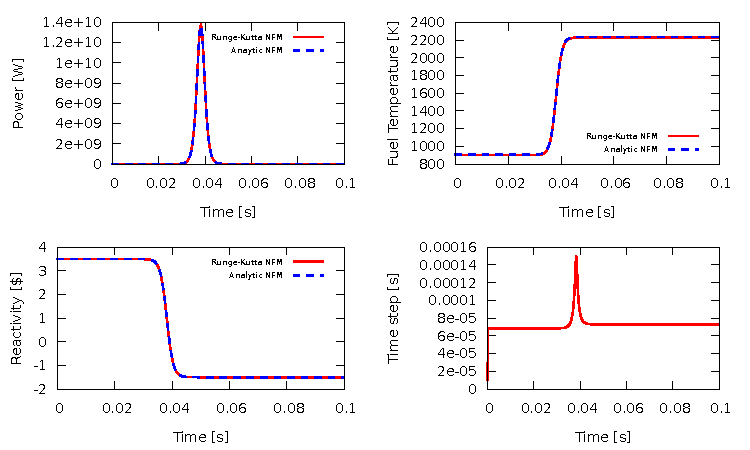
\includegraphics[scale=0.9]{./figs/nordheimfuchs.pdf}
\end{frame}

\begin{frame}{Point Kinetics w/ Feedback}
  \includegraphics[scale=0.9]{./figs/pkfeedback.pdf}
\end{frame}

%--------------------------------------------------------------------------------
\end{document}
